% Ball-screw feed axis, with section of a preloaded double nut
\documentclass[dvisvgm,tikz,border=4pt]{standalone}
% Shared preamble for the TikZ figures in images-1/src (compiled by build.sh)
\usepackage{helvet}
\renewcommand\familydefault{\sfdefault}
\usepackage{amsmath, amssymb}
\usetikzlibrary{arrows.meta, calc, decorations.pathreplacing, patterns, positioning, shapes.geometric, 3d, perspective, fit, backgrounds}
% palette shared with slides.scss and the Graphviz diagrams
\definecolor{dmred}{HTML}{880000}
\definecolor{dmblue}{HTML}{000088}
\definecolor{dmgreen}{HTML}{008800}
\definecolor{dmorange}{HTML}{E08A1E}
\definecolor{ink}{HTML}{333333}
\definecolor{fillblue}{HTML}{E8E8F8}
\definecolor{fillred}{HTML}{F3EAEA}
\definecolor{fillgreen}{HTML}{E8F4E8}
\definecolor{fillorange}{HTML}{FDF0DC}
\definecolor{steel}{HTML}{C9D3DC}
\definecolor{steeldk}{HTML}{8FA3B5}
\definecolor{metal}{HTML}{D9D9D9}
\definecolor{metaldk}{HTML}{A6A6A6}
\tikzset{
  >={Stealth[length=7pt]},
  every picture/.style={line cap=round, line join=round, font=\large},
  proj/.style={gray, dashed, thin},
  dim/.style={<->, >={Stealth[length=5pt]}, thin},
  ext/.style={very thin, gray},
  callout/.style={gray!70!black, thin},
  % datum (origin) symbol
  % pics use absolute sizes so they look the same in mm-scaled drawings
  datum/.pic={
    \fill[white] (0,0) circle (0.22cm);
    \fill[black] (0,0) -- ++(0.22cm,0) arc[start angle=0, end angle=-90, radius=0.22cm] -- cycle;
    \fill[black] (0,0) -- ++(-0.22cm,0) arc[start angle=180, end angle=90, radius=0.22cm] -- cycle;
    \draw[thick] (0,0) circle (0.22cm);
  },
  % reference symbols (absolute sizes): origins have a double circle with a filled quadrant
  wporigin/.pic={
    \draw[thick, fill=white] (0,0) circle (0.3cm);
    \fill[black] (0,0) -- (0.18cm,0) arc[start angle=0, end angle=-90, radius=0.18cm] -- cycle;
    \draw[thick] (0,0) circle (0.18cm);
    \draw (-0.3cm,0) -- (0.3cm,0) (0,-0.3cm) -- (0,0.3cm);
  },
  machorigin/.pic={
    \draw[thick, fill=white] (0,0) circle (0.3cm);
    \fill[black] (0,0) -- (-0.18cm,0) arc[start angle=180, end angle=90, radius=0.18cm] -- cycle;
    \draw[thick] (0,0) circle (0.18cm);
    \draw (-0.3cm,0) -- (0.3cm,0) (0,-0.3cm) -- (0,0.3cm);
  },
  supportpt/.pic={
    \draw[thick, fill=white] (0,0) circle (0.15cm);
    \draw (-0.15cm,0) -- (0.15cm,0) (0,-0.15cm) -- (0,0.15cm);
  },
  regpt/.pic={
    \draw[thick, fill=white] (0,0) circle (0.24cm);
    \draw[thick] (0,0) circle (0.15cm);
    \draw (-0.15cm,0) -- (0.15cm,0) (0,-0.15cm) -- (0,0.15cm);
  },
  % support / registration point (generic)
  target/.pic={
    \draw[thick, fill=white] (0,0) circle (0.12cm);
    \draw (-0.2cm,0) -- (0.2cm,0) (0,-0.2cm) -- (0,0.2cm);
  },
}

% Shared side-view components for the feed-drive figures (not compiled on its own)
\tikzset{
  part/.style={thick, fill=metal},
  screwbody/.style={thick, fill=metal!60, postaction={pattern=north west lines, pattern color=gray!80}},
  sensor/.style={thick, fill=dmgreen!30, draw=dmgreen!50!black},
  wire/.style={thick, dmblue, ->, rounded corners=3pt},
  power/.style={thick, ->, rounded corners=3pt},
}
% \screw{x1}{x2}{y}: lead screw along y (axis), radius 0.18
\newcommand\screw[3]{\draw[screwbody] (#1,#3-0.18) rectangle (#2,#3+0.18);}
% \shaft{x1}{x2}{y}
\newcommand\shaft[3]{\draw[thick, fill=metal!60] (#1,#3-0.1) rectangle (#2,#3+0.1);}
% \motor{x left}{y axis}: body 1.4 x 1.0, shaft to the right
\newcommand\motor[2]{%
  \draw[part, fill=metaldk!60, rounded corners=2pt] (#1,#2-0.5) rectangle (#1+1.4,#2+0.5);
  \foreach \i in {1,...,5} \draw[gray!60!black] (#1+0.22*\i,#2-0.5) -- (#1+0.22*\i,#2+0.5);
  \draw[part] (#1+1.4,#2-0.3) rectangle (#1+1.55,#2+0.3);}
% \bearing{x}{y}: support bearing around the screw
\newcommand\bearing[2]{%
  \draw[part, fill=metal!80] (#1-0.18,#2+0.18) rectangle (#1+0.18,#2+0.5);
  \draw[part, fill=metal!80] (#1-0.18,#2-0.5) rectangle (#1+0.18,#2-0.18);
  \draw (#1-0.18,#2+0.18) -- (#1+0.18,#2+0.5) (#1-0.18,#2+0.5) -- (#1+0.18,#2+0.18);
  \draw (#1-0.18,#2-0.5) -- (#1+0.18,#2-0.18) (#1-0.18,#2-0.18) -- (#1+0.18,#2-0.5);}
% \coupling{x}{y}
\newcommand\coupling[2]{\draw[part, fill=metaldk!40] (#1-0.18,#2-0.28) rectangle (#1+0.18,#2+0.28);}
% \rotenc{x}{y}: rotary encoder disk seen edge-on
\newcommand\rotenc[2]{\draw[sensor] (#1-0.09,#2-0.45) rectangle (#1+0.09,#2+0.45);}
% \tablenut{x centre}{y axis}{half length}: table with nut on the screw
\newcommand\tablenut[3]{%
  \draw[part, fill=dmorange!55] (#1-#3,#2+0.6) rectangle (#1+#3,#2+1.1);
  \draw[part, fill=dmorange!35] (#1-0.4,#2-0.3) rectangle (#1+0.4,#2+0.6);}

\begin{document}
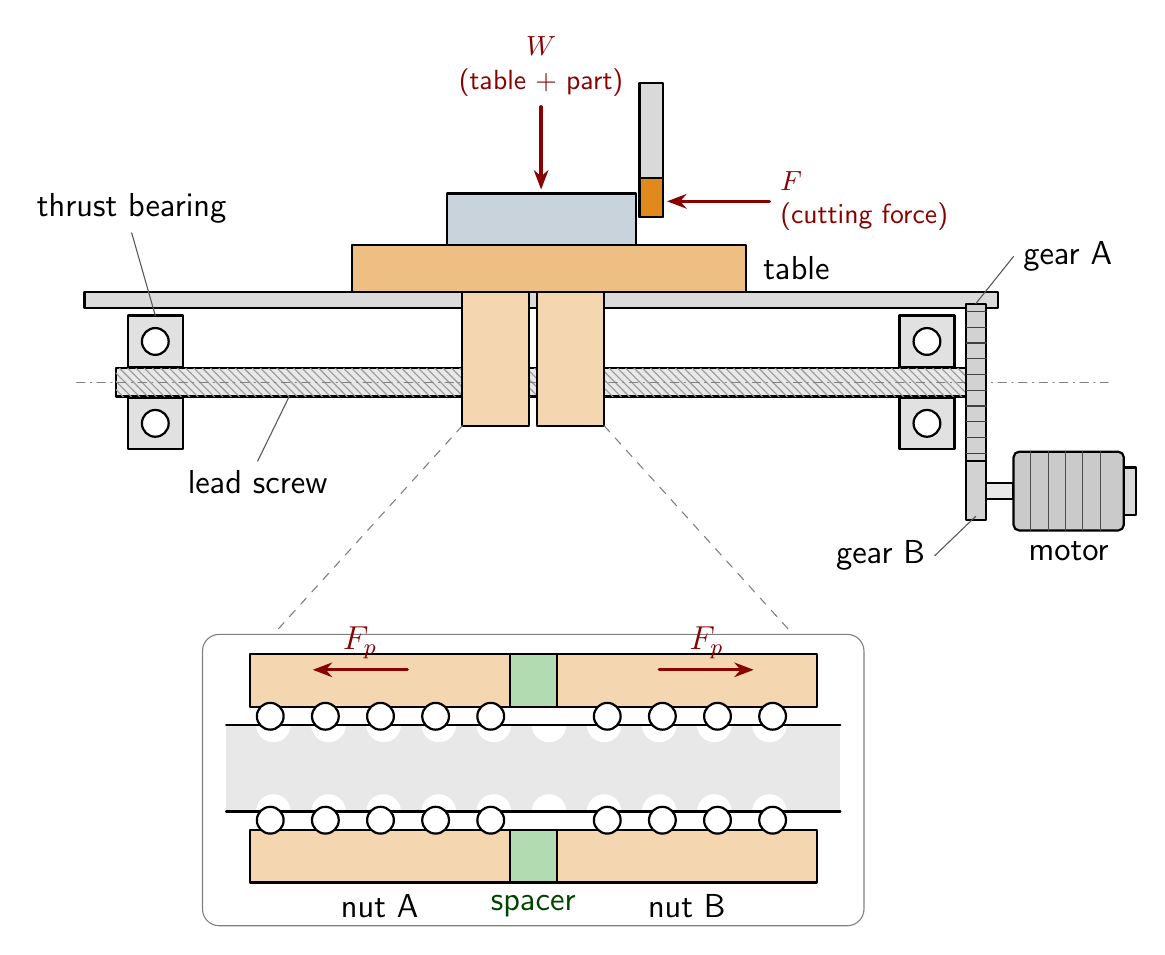
\begin{tikzpicture}[font=\large]
  % ---------------- axis
  \screw{0.2}{11.0}{0}
  \draw[dash dot, gray] (-0.3,0) -- (12.8,0);
  % angular-contact thrust bearings at both ends
  \foreach \x in {0.7, 10.5}{
    \draw[part, fill=metal!80] (\x-0.35,0.2) rectangle (\x+0.35,0.85);
    \draw[part, fill=metal!80] (\x-0.35,-0.85) rectangle (\x+0.35,-0.2);
    \foreach \s in {1,-1} \draw[thick, fill=white] (\x,{\s*0.52}) circle (0.17);
  }
  % guideways, table and double nut
  \draw[part, fill=metaldk!40] (-0.2,0.95) rectangle (11.4,1.15);
  \draw[part, fill=dmorange!55] (3.2,1.15) rectangle (8.2,1.75);
  \draw[part, fill=dmorange!35] (4.6,-0.55) rectangle (5.45,1.15);
  \draw[part, fill=dmorange!35] (5.55,-0.55) rectangle (6.4,1.15);
  % workpiece, tool and loads
  \draw[part, fill=steel] (4.4,1.75) rectangle (6.8,2.4);
  \draw[part, fill=metal] (6.85,2.1) rectangle (7.15,3.8);
  \draw[part, fill=dmorange] (6.85,2.1) rectangle (7.15,2.6);
  \draw[->, very thick, dmred] (8.5,2.3) -- (7.2,2.3) node[pos=0, right, align=left, font=\normalsize] {$F$\\(cutting force)};
  \draw[->, very thick, dmred] (5.6,3.5) -- (5.6,2.45) node[pos=0, above, align=center, font=\normalsize] {$W$\\(table + part)};
  % gear pair and motor at the right end
  \draw[part, fill=metaldk!50] (11.0,-1.0) rectangle (11.25,1.0);
  \draw[part, fill=metaldk!50] (11.0,-1.75) rectangle (11.25,-1.0);
  \foreach \y in {-0.9,-0.7,...,0.9} \draw[gray!50!black] (11.0,\y) -- (11.25,\y);
  \shaft{11.25}{11.6}{-1.38}
  \motor{11.6}{-1.38}
  % labels
  \draw[callout] (0.7,0.85) -- (0.4,1.9) node[above, black] {thrust bearing};
  \draw[callout] (2.4,-0.18) -- (2.0,-1.0) node[below, black] {lead screw};
  \draw[callout] (11.12,1.0) -- (11.6,1.6) node[right, black] {gear A};
  \draw[callout] (11.12,-1.7) -- (10.6,-2.2) node[left, black] {gear B};
  \node[below] at (12.3,-1.9) {motor};
  \node[right] at (8.3,1.45) {table};
  % ---------------- inset: preloaded double nut in section
  \draw[dashed, gray] (4.6,-0.55) -- (2.2,-3.2) (6.4,-0.55) -- (8.8,-3.2);
  \begin{scope}[shift={(5.5,-4.9)}]
    \draw[gray, rounded corners=6pt] (-4.2,-2.0) rectangle (4.2,1.7);
    % screw core with ball grooves
    \fill[metal!60] (-3.9,-0.55) rectangle (3.9,0.55);
    \foreach \x in {-3.3,-2.6,...,3.4}{
      \fill[white] (\x,0.55) circle (0.22) (\x,-0.55) circle (0.22);}
    \draw[thick] (-3.9,0.55) -- (3.9,0.55) (-3.9,-0.55) -- (3.9,-0.55);
    % nut halves (A, B) with spacer, upper and lower section
    \foreach \s in {1,-1}{
      \draw[part, fill=dmorange!35] (-3.6,{\s*0.78}) rectangle (-0.3,{\s*1.45});
      \draw[part, fill=dmorange!35] (0.3,{\s*0.78}) rectangle (3.6,{\s*1.45});
      \draw[part, fill=dmgreen!30] (-0.3,{\s*0.78}) rectangle (0.3,{\s*1.45});
    }
    % balls: nut A loaded on the left flanks, nut B on the right flanks
    \foreach \x in {-3.3,-2.6,-1.9,-1.2,-0.5}{
      \draw[thick, fill=white] (\x-0.04,0.66) circle (0.17) (\x-0.04,-0.66) circle (0.17);}
    \foreach \x in {0.9,1.6,2.3,3.0}{
      \draw[thick, fill=white] (\x+0.04,0.66) circle (0.17) (\x+0.04,-0.66) circle (0.17);}
    \draw[->, very thick, dmred] (-1.6,1.25) -- node[above] {$F_p$} (-2.8,1.25);
    \draw[->, very thick, dmred] (1.6,1.25) -- node[above] {$F_p$} (2.8,1.25);
    \node at (-1.95,-1.75) {nut A};
    \node at (1.95,-1.75) {nut B};
    \node[dmgreen!50!black] at (0,-1.75) {spacer};
  \end{scope}
\end{tikzpicture}
\end{document}
